\section{Simulation Environment}
\label{sec:SimEnvironment}

The experimental investigation is conducted using the open-source \ac{sumo} framework, selected for its high-fidelity microscopic vehicle dynamics and its capacity for deterministic reproducibility. All simulation inputs are provided via static configuration files to ensure consistency, with no on-line calibration performed during the runs. The platform's default numerical integration solver is used for all calculations.
\mynewline
The simulation network is a high-fidelity digital twin of the signalised \emph{Neckartor} junction in Stuttgart, a location known for heavy traffic and previous environmental studies. Figure~\vref{fig:NeckartorMapComparison} provides a direct visual comparison of the junction. The satellite imagery in Figure~\vref{fig:NeckartorMapReal} shows the complex real-world geometry, which is precisely replicated in the \ac{sumo} environment, as depicted in Figure~\vref{fig:NeckartorMapSUMO}. This includes all lane layouts and dedicated turn pockets. Signal control is governed by fixed \ac{spat} and \ac{map} plans extracted from the actual roadside controller, which are assumed to be invariant throughout each simulation run. In accordance with local traffic regulations, the vehicle fleet excludes diesel vehicles that do not meet the Euro 6 standard, mirroring the driving ban on older, more polluting models. The simulation's traffic demand is anchored to empirical data, with measured vehicle counts from 2023 indicating a peak flow of $2800\unit{\veh\per\hour}$.
\mynewline

\begin{figure}[htb]
  \centering
  \begin{subfigure}[b]{0.49\textwidth}
    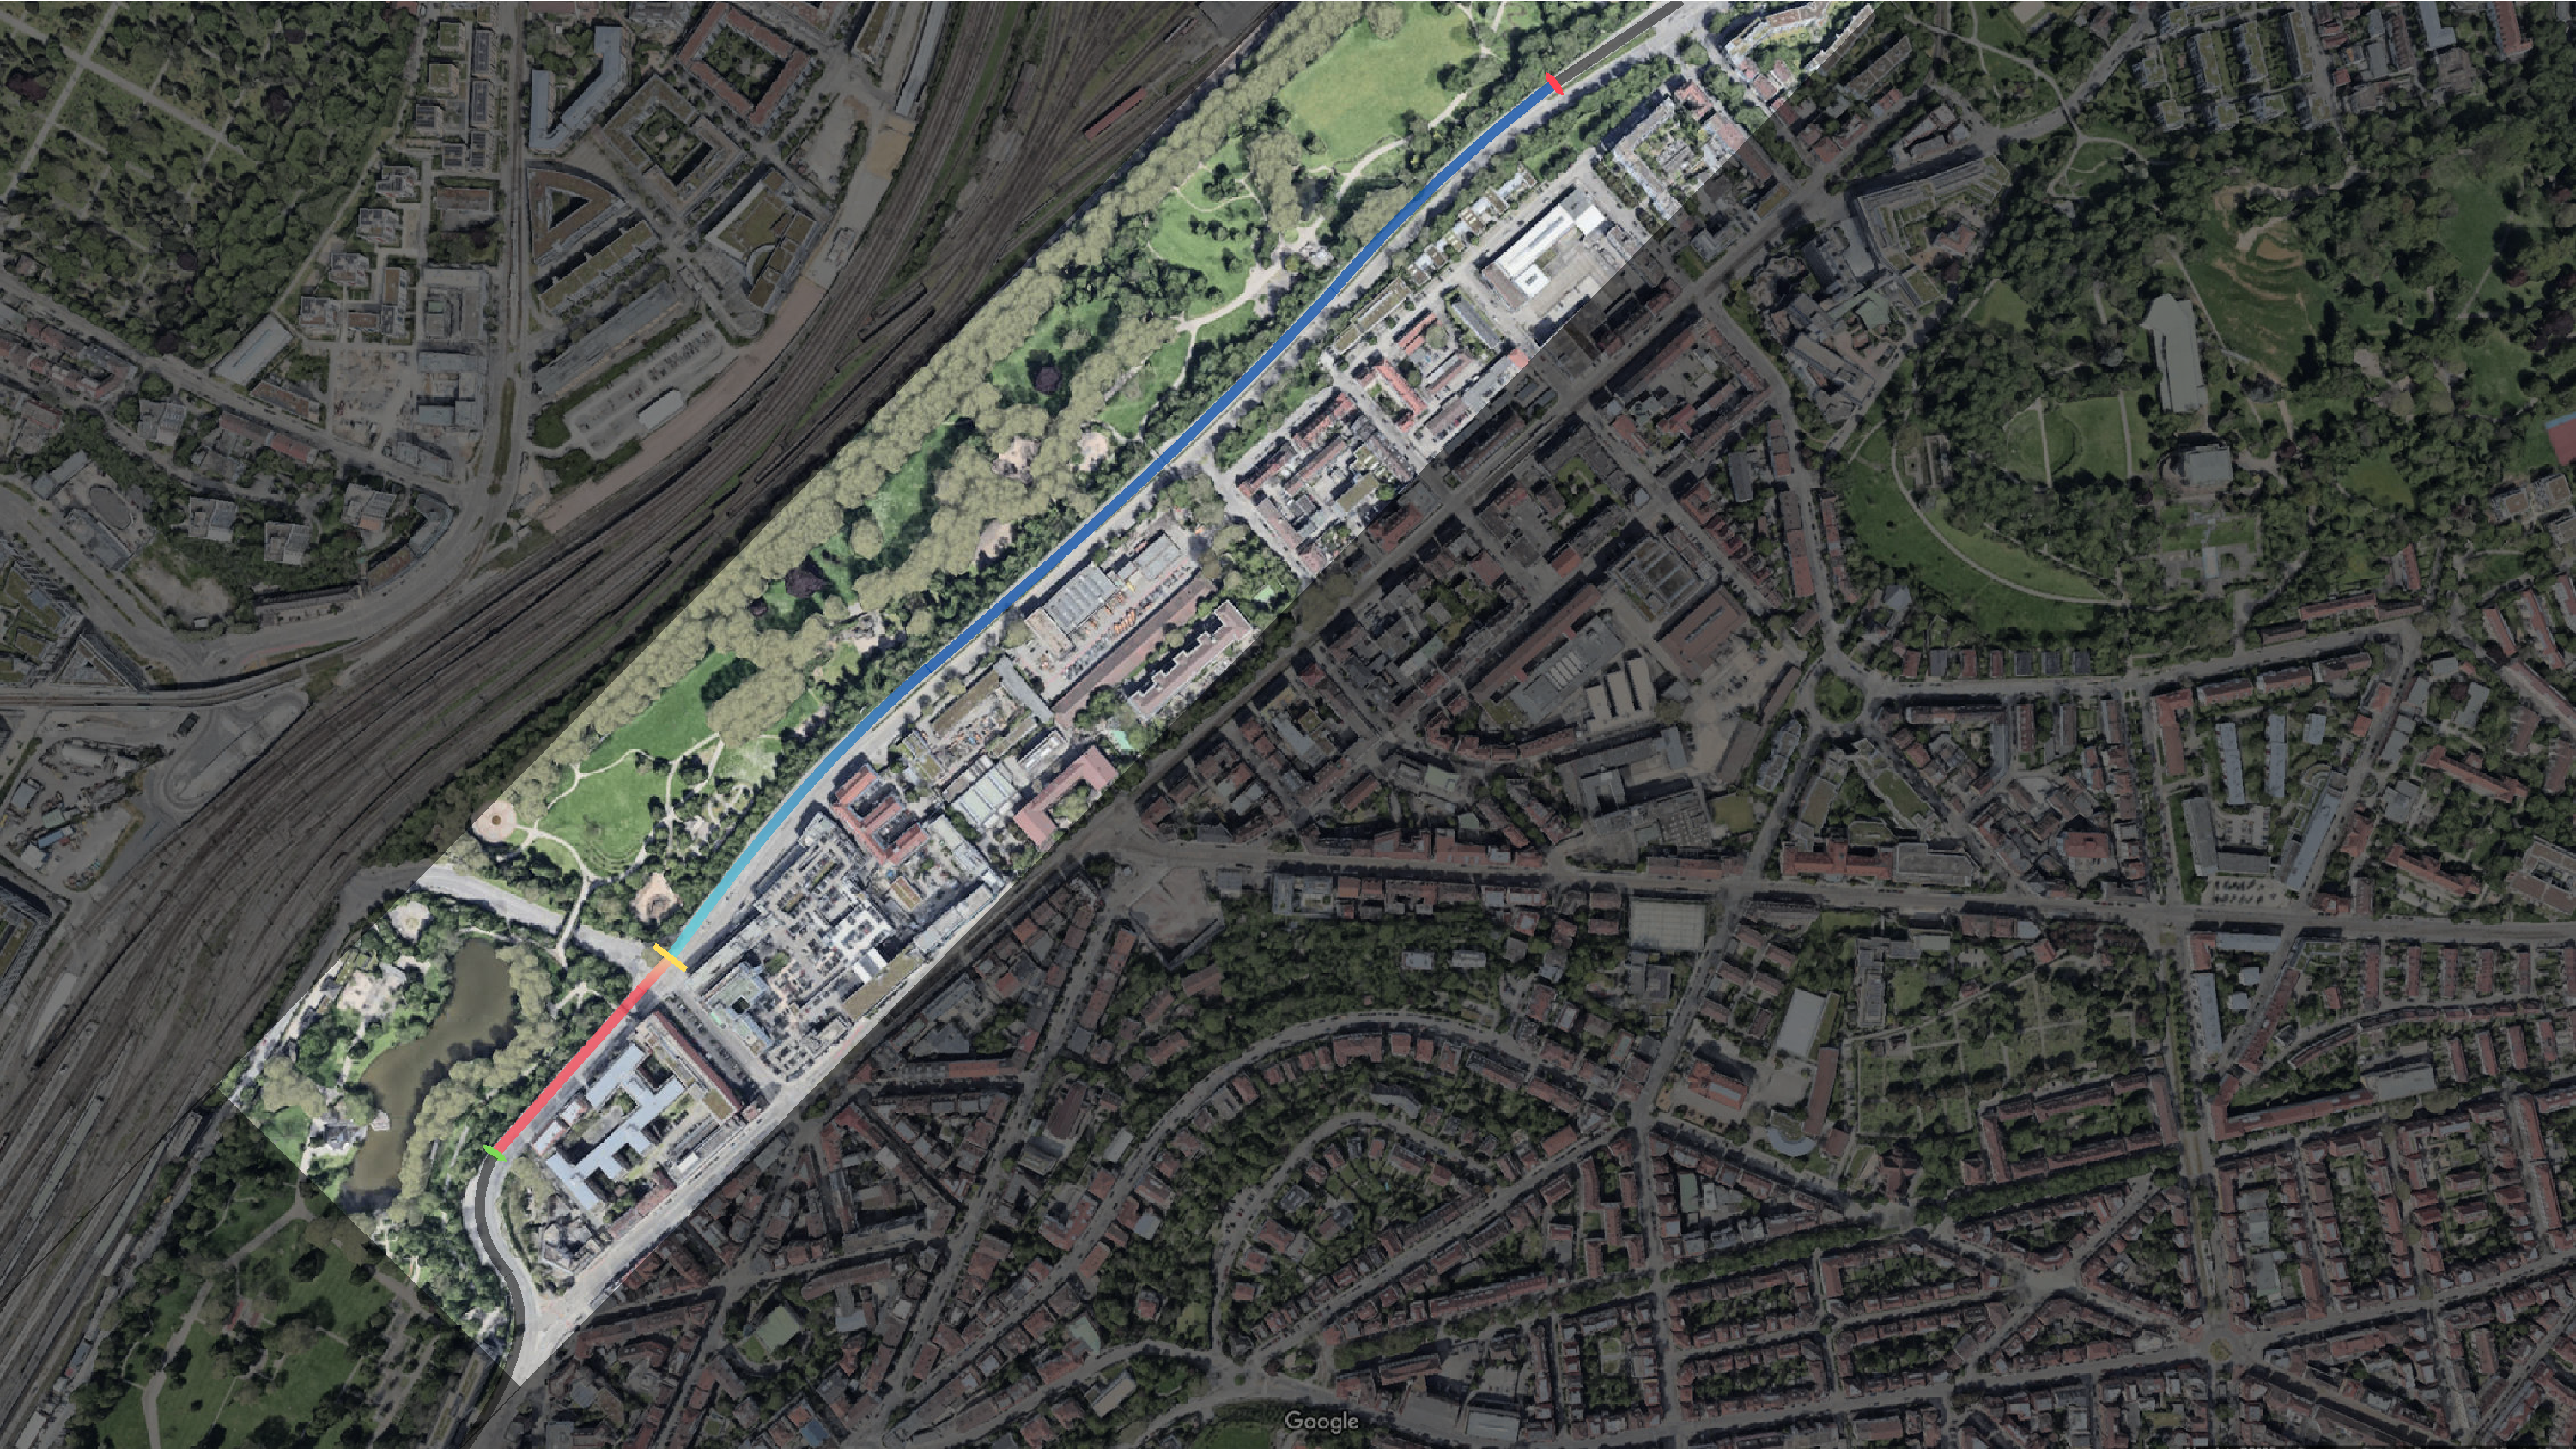
\includegraphics[width=\linewidth, page=1]{data/img/Neckartor/StuttgartNeckartorReal.pdf}
    \caption[Neckartor junction satellite image]{Satellite imagery of the real-world Neckartor junction in Stuttgart, highlighting the complex geometry and surrounding urban environment.}
    \label{fig:NeckartorMapReal}
  \end{subfigure}
  \hfill
  \begin{subfigure}[b]{0.49\textwidth}
    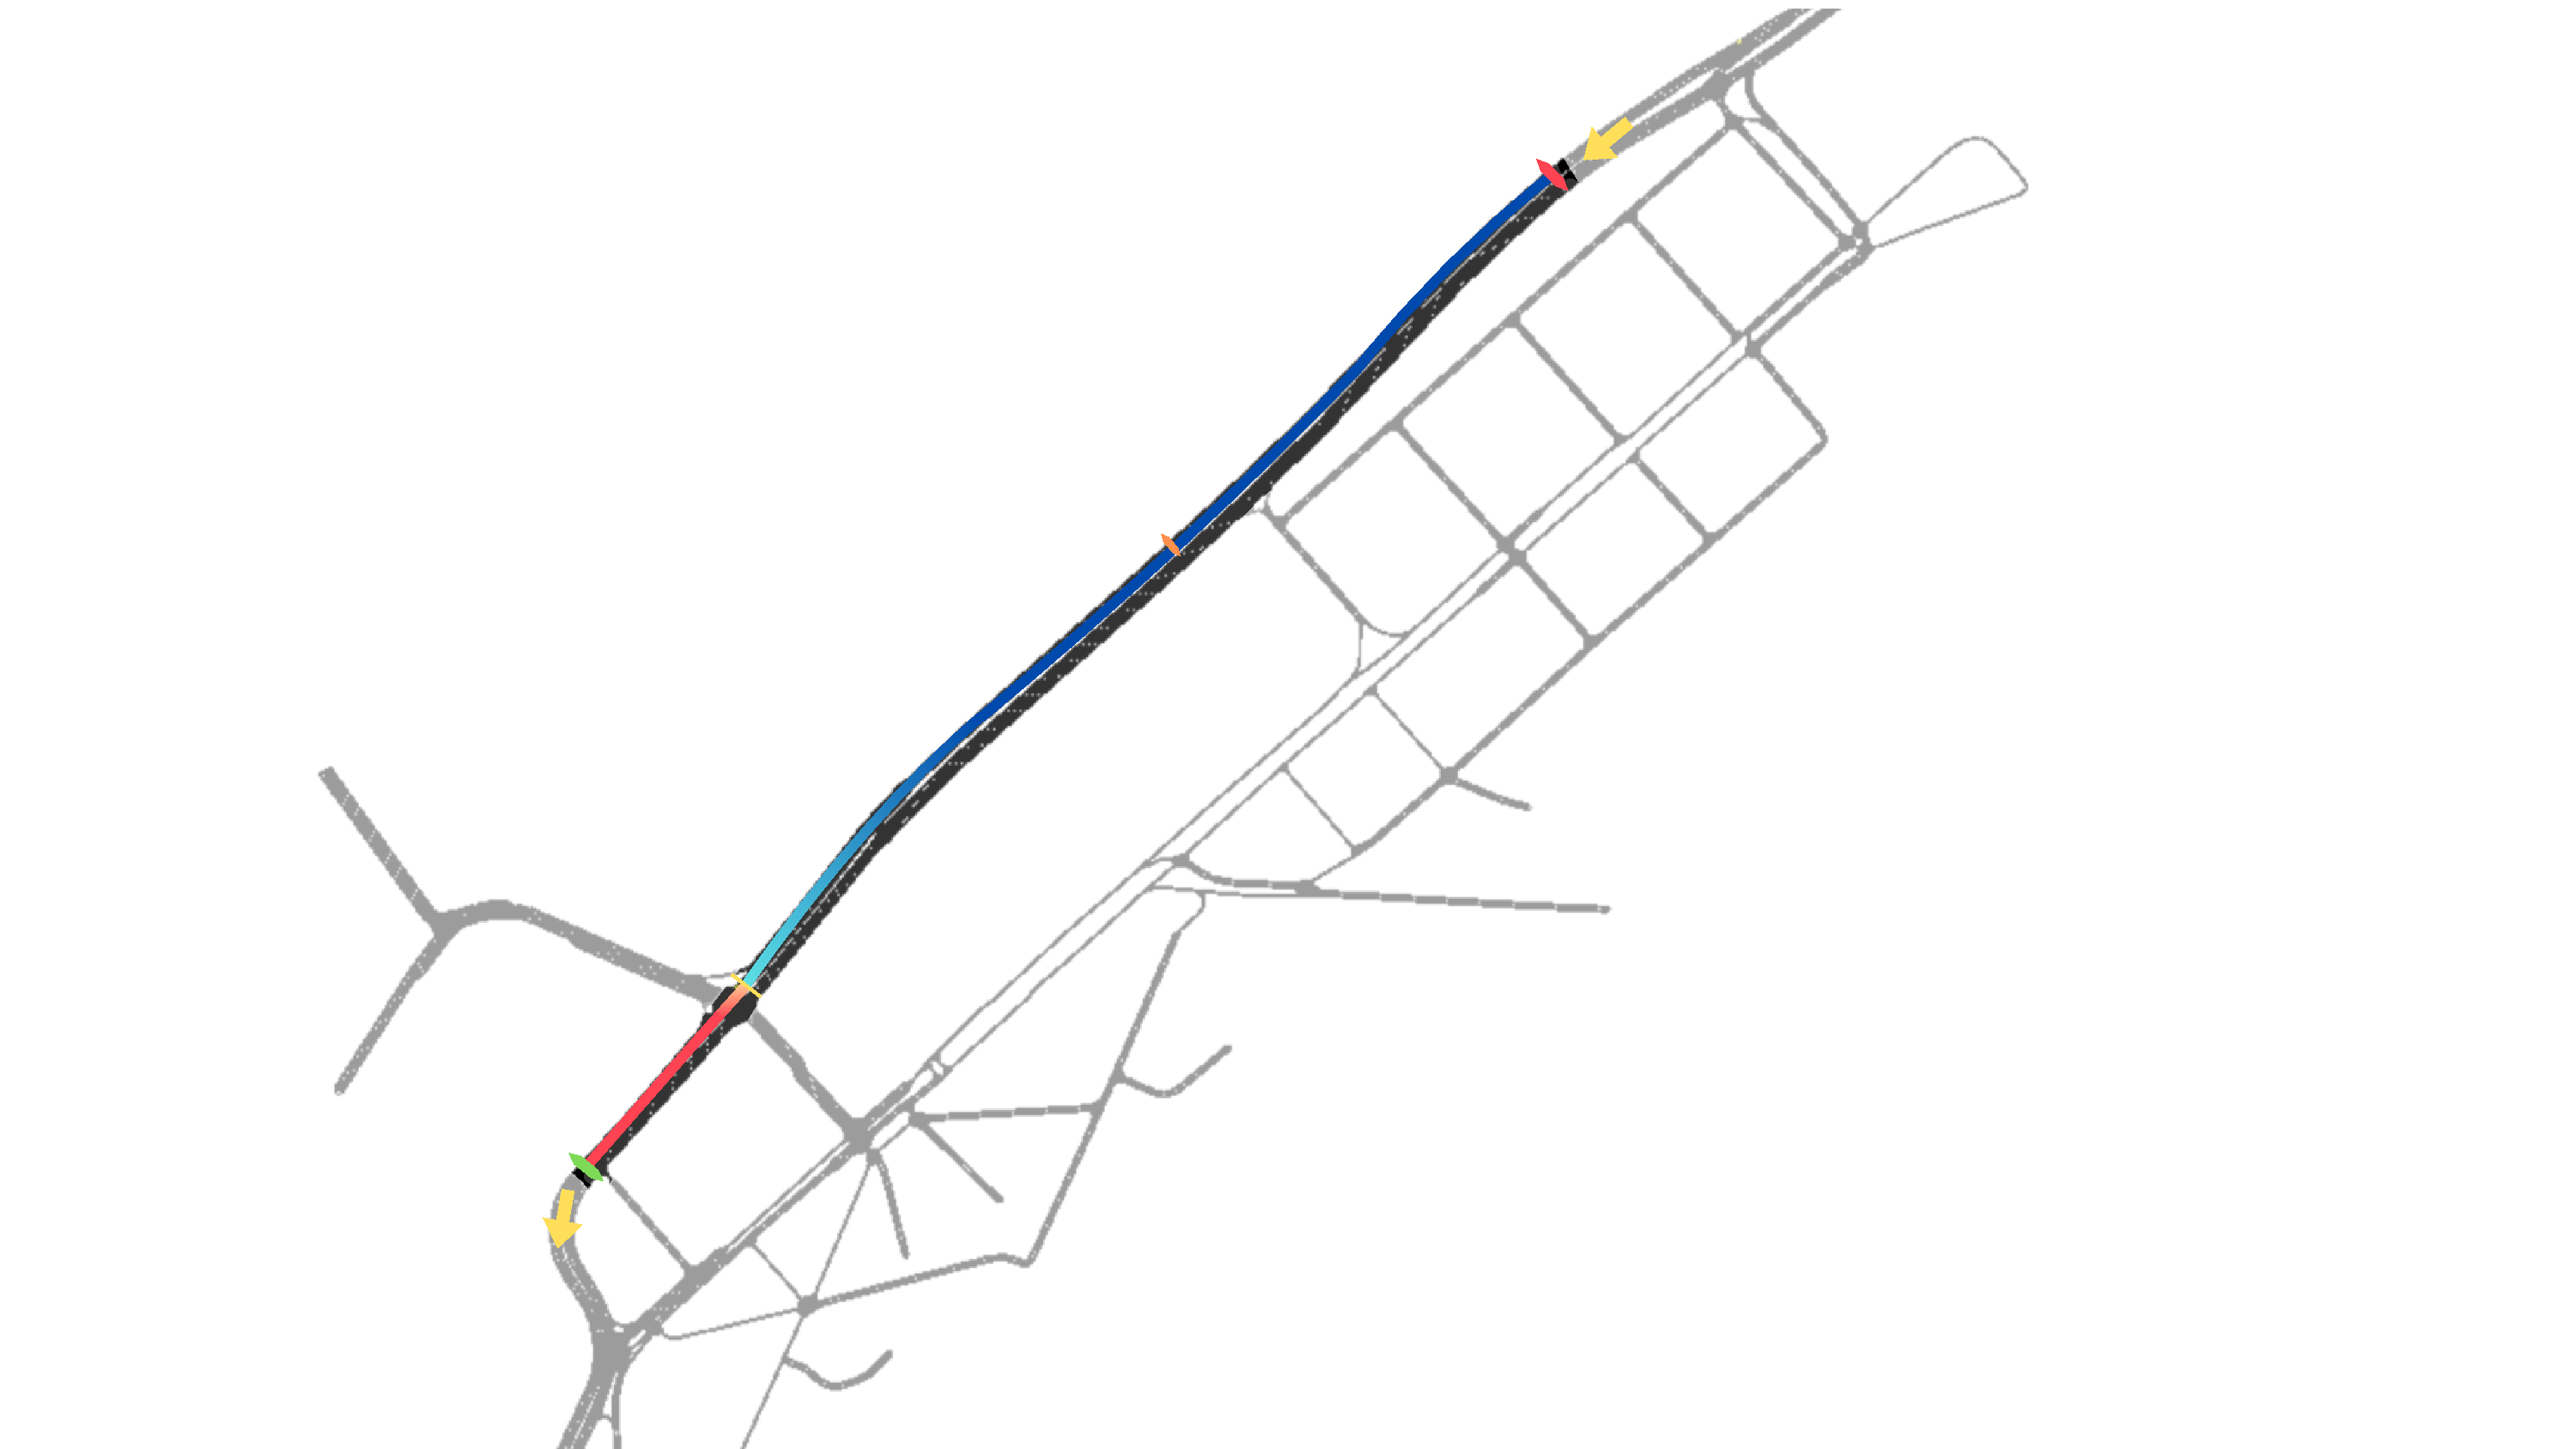
\includegraphics[width=\linewidth, page=1]{data/img/Neckartor/StuttgartNeckartorSumo.pdf}
    \caption[Digital twin of Neckartor in \ac{sumo}]{The digital twin of the Neckartor junction as implemented in the \ac{sumo} environment, showing the modelled lanes and connections.}
    \label{fig:NeckartorMapSUMO}
  \end{subfigure}
  \caption[Real-World vs. Simulated Neckartor Junction]{%
  Comparison of the real-world Neckartor junction (left) with its high-fidelity digital twin in the \ac{sumo} simulation (right). 
  The red segment marks the downstream cordon, while the blue segment indicates the upstream cordon. 
  The yellow line represents the signalized intersection. 
  Red square dots denote the start points for the $1000\unit{\metre}$ downstream advisory range, while orange square dots denote the start points for the $500\unit{\metre}$ range. 
  The green square marks the corresponding upstream end point of each advisory range. 
  Yellow arrows indicate the driving direction in each lane.}
  \label{fig:NeckartorMapComparison}
\end{figure}

Traffic demand is generated synthetically but is anchored to real-world loop detector data from the B14 corridor. The generated flow levels span the full spectrum of traffic states, from light, uncongested conditions to heavy, oversaturated congestion. Within each scenario, vehicles are introduced into the network with uniform inter-arrival times. Route assignment follows an equal probability distribution across all legitimate movements to ensure a balanced saturation of all lane groups. The \ac{glosa} \ac{mpr} is treated as a primary experimental variable, systematically tested in $10\%$ increments from $0\%$ (no equipped vehicles) to $100\%$ (fully equipped fleet). To manage this, two statistically independent insertion streams are used, allowing \ac{glosa}-equipped and non-equipped vehicles to coexist and interact within the same network environment.
\mynewline
The longitudinal driving behaviour for all vehicles is governed by the \ac{eidm}, a model chosen for its demonstrated ability to realistically capture stop-and-go waves and queue discharge dynamics. To ensure the simulation reflects real-world driver diversity, a heterogeneous fleet is synthesized by defining a combination of eleven fixed and eleven variable vehicle parameters. The fixed parameters, which establish baseline physical and behavioural constraints for all vehicles, are detailed in Table~\vref{tab:FixedFleetParams}. The variable parameters, listed in Table~\vref{tab:VariableFleetParams}, are sampled independently of uniform distributions over their specified ranges for each vehicle at spawn time. This methodology produces a rich vehicle population with a plausible span of physical dimensions (e.g., length and width) and driver characteristics (e.g., aggressiveness, reaction time), preventing a bias towards any single calibration point.
\mynewline

\begin{table}[htb]
  \centering
  \caption[Variable Vehicle Fleet Parameters]{Variable vehicle parameters used to synthesize the heterogeneous fleet in \ac{sumo}. Each parameter is drawn independently of a uniform distribution over the specified range at vehicle spawn time to ensure a realistic mix of driver behaviours and vehicle types. Derived from Lenz \cite{Lenz2024}.}
  \label{tab:VariableFleetParams}
  \resizebox{\textwidth}{!}{%
    \begin{tabular}{l l c c}
      \toprule
      \textbf{Parameter} & \textbf{Explanation} & \textbf{Min Value} & \textbf{Max Value} \\
      \midrule
      minGap & Minimum vehicle gap at standstill & $0.5\unit{m}$ & $4\unit{m}$ \\
      accel & Maximum acceleration & $0.97\unit{m\,s^{-2}}$ & $4\unit{m\,s^{-2}}$ \\
      startupDelay & Time delay until vehicle starts moving & $0.0\unit{s}$ & $2.0\unit{s}$ \\
      tau & Time headway maintained to the preceding vehicle & $0.5\unit{s}$ & $1.5\unit{s}$ \\
      delta & Influences how the vehicle reacts to speed differences & $1.0$ & $4.97$ \\
      treaction & Driver's reaction time & $0.2\unit{s}$ & $0.9\unit{s}$ \\
      tacmax & Time the vehicle needs to reach maximum acceleration & $0.5\unit{s}$ & $3.0\unit{s}$ \\
      Mflatness & \enquote{Flatness} of the acceleration and deceleration behavior & $1.0$ & $5.0$ \\
      Mbegin & Parameter for starting behavior & $0.1$ & $1.49$ \\
      length & Length of the vehicle & $2.2\unit{m}$ & $9.3\unit{m}$ \\
      width & Width of the vehicle & $1.5\unit{m}$ & $2.5\unit{m}$ \\
      \bottomrule
    \end{tabular}%
  }
\end{table}

\begin{table}[htb]
  \centering
  \caption[Fixed Vehicle Fleet Parameters]{Fixed vehicle parameters shared by all vehicles in the simulation fleet. These values define baseline behaviours and physical constraints, ensuring consistent dynamics across the entire population. Derived from Lenz \cite{Lenz2024}.}
  \label{tab:FixedFleetParams}
  \resizebox{\textwidth}{!}{%
    \begin{tabular}{l l c}
      \toprule
      \textbf{Parameter} & \textbf{Explanation} & \textbf{Value} \\
      \midrule
      decel & Maximum deceleration & $2.5\unit{m\,s^{-2}}$ \\
      emergencyDecel & Maximum emergency braking deceleration & $15\unit{m\,s^{-2}}$ \\
      tpreview & Time horizon a vehicle "looks" into the future to plan speed & $4\unit{s}$ \\
      tPersDrive & Duration the vehicle remains in continuous driving mode & $3\unit{s}$ \\
      tPersEstimate & Duration the vehicle remains in estimation mode & $10\unit{s}$ \\
      coolness & Influences how calmly or aggressively a vehicle reacts to disturbances & $0.99$ \\
      signaleader & Inaccuracy of speed adaptation to the preceding vehicle & $0.02$ \\
      sigmaerror & Inaccuracy regarding errors in driving style (speed, distance) & $0.1$ \\
      sigmagap & Inaccuracy of the gap to the preceding vehicle & $0.1$ \\
      jerkmax & Maximum rate of change of acceleration & $3\unit{m\,s^{-3}}$ \\
      epsilonacc & Inaccuracy of acceleration estimation & $1.0$ \\
      \bottomrule
    \end{tabular}%
  }
\end{table}

Each simulation is run for a total temporal horizon of $43.33\unit{min}$. The initial $10\unit{min}$ of this period serves as a warm-up phase, which allows traffic flows to stabilize and ensures that initial transient effects do not influence the results. Consequently, only data from the final $33.33\,\unit{min}$ are used for statistical analysis. A simulation time step of $0.1\unit{s}$ is maintained to provide sufficient resolution for both the \ac{eidm}'s dynamic equations and for the accurate integration of instantaneous emissions. For data collection, the analysis is spatially constrained to a corridor extending $1\unit{km}$ upstream and $200\,\unit{m}$ downstream from the intersection's primary stop line. This spatial clipping focuses the evaluation on the region most directly influenced by the \ac{glosa} advisories.
\mynewline
For each simulated vehicle, a dedicated log file is generated that records a high-resolution time series of its state, including timestamp, position, speed, and acceleration. Instantaneous emission rates for all relevant pollutants are concurrently calculated using \ac{sumo}’s internal emission model back-ends. To facilitate post-processing with external analysis scripts, these logs are flushed at every simulation step. A consistent configuration is applied across all scenarios to ensure the comparability of results throughout the comprehensive sweeps of traffic flow, market penetration, and other experimental parameters.

